\begin{center}
\section{Assignment: Search fixed target using the ultrasonic Sensor}
%\addcontentsline{toc}{section}{\protect\numberline{}Search fixed target using the ultrasonic Sensor.}%
\end{center}
\label{sec:first-n-follow}

\subsection{Introduction}
%\addcontentsline{toc}{subsection}{\protect\numberline{Introduction}}%

The quest for precision and efficiency in autonomous navigation and detection has driven the development of cutting-edge technologies, with ultrasonic sensors emerging as a crucial tool. This simulation endeavors to explore the capabilities of an ultrasonic sensor for targeted distance measurements in a two-dimensional plane, echoing real-world scenarios where such sensors find application.

In this simulation, we emulate the behavior of an ultrasonic sensor that discerns distances to the nearest reflective target within a predefined two-dimensional cone. This cone is characterized by its apex at the sensor's location, its axis perpendicular to the sensor's face, and a constant opening angle that determines the beam's width or aperture.

\subsubsection{Ultrasonic Beam Definition}
%\addcontentsline{toc}{subsubsection}{\protect\numberline{Ultrasonic Beam Definition}}%Ultrasonic Beam Definition

The ultrasonic sensor's behavior is analogous to radar-like detection, as it generates a beam that extends outwards from its position. This beam covers an area defined by the cone, with its range limited to the nearest reflecting object. To facilitate this process, we introduce the concept of "targets." Targets are polygonal shapes detectable through a mesh of triangles emanating from their center point. While these targets have attributed sprite images, their visual representation isn't utilized for the detection process.

The essence of the distance detection algorithm lies in the mesh of triangles, with the algorithm providing the distance to the nearest triangle within the sensor's beam area. Crucially, the number of targets is not constrained, allowing for dynamic creation and modification of targets during runtime.

In practical application, establishing a fixed target layout can be achieved through the \texttt{RobotContext} class. By mirroring real-world scenarios, this approach ensures that code for robot movement remains consistent regardless of whether it's applied in direct interaction or autonomous mode. In the context of this simulation, a robot employs a radar-like movement pattern to search for a target. Once detected, the robot navigates towards the target and halts at a predefined distance.

This simulation affords a window into the potential of ultrasonic sensors in navigating complex environments, and the subsequent sections will delve deeper into the mechanics and implications of this technology.

\subsection{Methodology}
%\addcontentsline{toc}{subsection}{\protect\numberline{Methodology}}

The provided Java code implements a simulation of a robot using an ultrasonic sensor to search for and approach a fixed target. The robot navigates within an environment using predefined movements and interactions with the ultrasonic sensor to accomplish its task.

Here's a breakdown of the methodology and key components of the code:

\begin{enumerate}
  \item \textbf{Import Statements:}
  \begin{itemize}
    \item The necessary libraries are imported, including \texttt{ch.aplu.robotsim.*} for the robot simulation environment and \texttt{java.awt.*} for graphics-related functionalities.
  \end{itemize}
  
  \item \textbf{Class Definition:}
  \begin{itemize}
    \item The \texttt{UltraSonicTarget} class is defined, which encapsulates the entire functionality of the program.
  \end{itemize}
  
  \item \textbf{Constructor:}
  \begin{itemize}
    \item The constructor \texttt{UltraSonicTarget()} initializes the robot, sets up its components, and executes the \texttt{runRobotProgram()} method.
  \end{itemize}
  
  \item \textbf{Robot Initialization:}
  \begin{itemize}
    \item An instance of \texttt{TurtleRobot} is created to simulate the robot.
    \item An instance of \texttt{Gear} is created to control the robot's movement.
    \item The speed of the gear is set to 10.
    \item An instance of \texttt{UltrasonicSensor} is created and attached to the robot's sensor port \texttt{S1}.
    \item The colors of the ultrasonic sensor's beam area and proximity circle are optionally configured.
  \end{itemize}
  
  \item \textbf{Main Robot Program (\texttt{runRobotProgram()}):}
  \begin{itemize}
    \item The \texttt{searchTarget()} method is called to initiate the robot's search for the target.
    \item A loop continuously checks the ultrasonic sensor's reading. If the distance to the target is less than 50, the robot stops its movement.
  \end{itemize}
  
  \item \textbf{Target Search (\texttt{searchTarget()}):}
  \begin{itemize}
    \item The robot employs a search pattern by moving right at a speed of 50.
    \item The ultrasonic sensor's distance reading is obtained.
    \item If a valid distance reading is received (not equal to -1), the robot turns right by 1500 units and starts moving forward toward the target. The search function is then exited.
  \end{itemize}
  
  \item \textbf{Main Method (\texttt{main()}):}
  \begin{itemize}
    \item The \texttt{UltraSonicTarget} class is instantiated, creating an instance of the robot and initiating the program.
  \end{itemize}
  
  \item \textbf{Environment Setup (Static Block):}
  \begin{itemize}
    \item The \texttt{RobotContext.useTarget()} method sets up the environment by loading a target image and defining a mesh of points to represent the target's shape. The target is placed at coordinates (350, 350) within the simulation environment.
  \end{itemize}
\end{enumerate}


\subsection{Code}
%\addcontentsline{toc}{subsection}{\protect\numberline{Code}}%

\label{subsec:code-first-n-follow}
\href{https://github.com/Mithunprb/MSc-Practicals-Journals/tree/main/MSc-Part2/Robotics/Assignment/src}{https://github.com/Mithunprb/MSc-Practicals-Journals/tree/main/MSc-Part2/Robotics/Assignment/src}  \\

\begin{minted}[mathescape, linenos, bgcolor=bg, frame=lines, framesep=2mm]{java}
/*
Search fixed target using the ultrasonic Sensor
 */
package ultrasonictarget;
import ch.aplu.robotsim.*;
import java.awt.*;

public class UltraSonicTarget
{
  private LegoRobot robot;
  private Gear gear;
  private UltrasonicSensor us;

  public UltraSonicTarget()
  {
    robot = new TurtleRobot();
    gear = new Gear();
    robot.addPart(gear);
    gear.setSpeed(10);
    us = new UltrasonicSensor(SensorPort.S1);
    robot.addPart(us);
    us.setBeamAreaColor(Color.green);  // May be commented out
    us.setProximityCircleColor(Color.lightGray); // May be commented out
    runRobotProgram();
  }

  private void runRobotProgram()
  {
    searchTarget();
    while (true)
    {
      if (us.getDistance() < 50)
        gear.stop();
    }
  }

  private void searchTarget()
  {
    while (true)
    {
      gear.right(50);
      int distance = us.getDistance();
      if (distance != -1)
      {
        gear.right(1500);
        gear.forward();
        return;
      }
    }
  }

  public static void main(String[] args)
  {
    new UltraSonicTarget();
  }

  // ------------------ Environment --------------------------
  static
  {
    Point[] mesh =
    {
      new Point(50, 0), new Point(25, 42), new Point(-25, 42),
      new Point(-50, 0), new Point(-25, -42), new Point(25, -42)
    };

    RobotContext.useTarget("sprites/target_red.gif", mesh, 350, 350);
  }
}
\end{minted}
\newpage
\subsection{Result}
%\addcontentsline{toc}{subsection}{\protect\numberline{Result}}%


\begin{figure}[h]
  \centering
  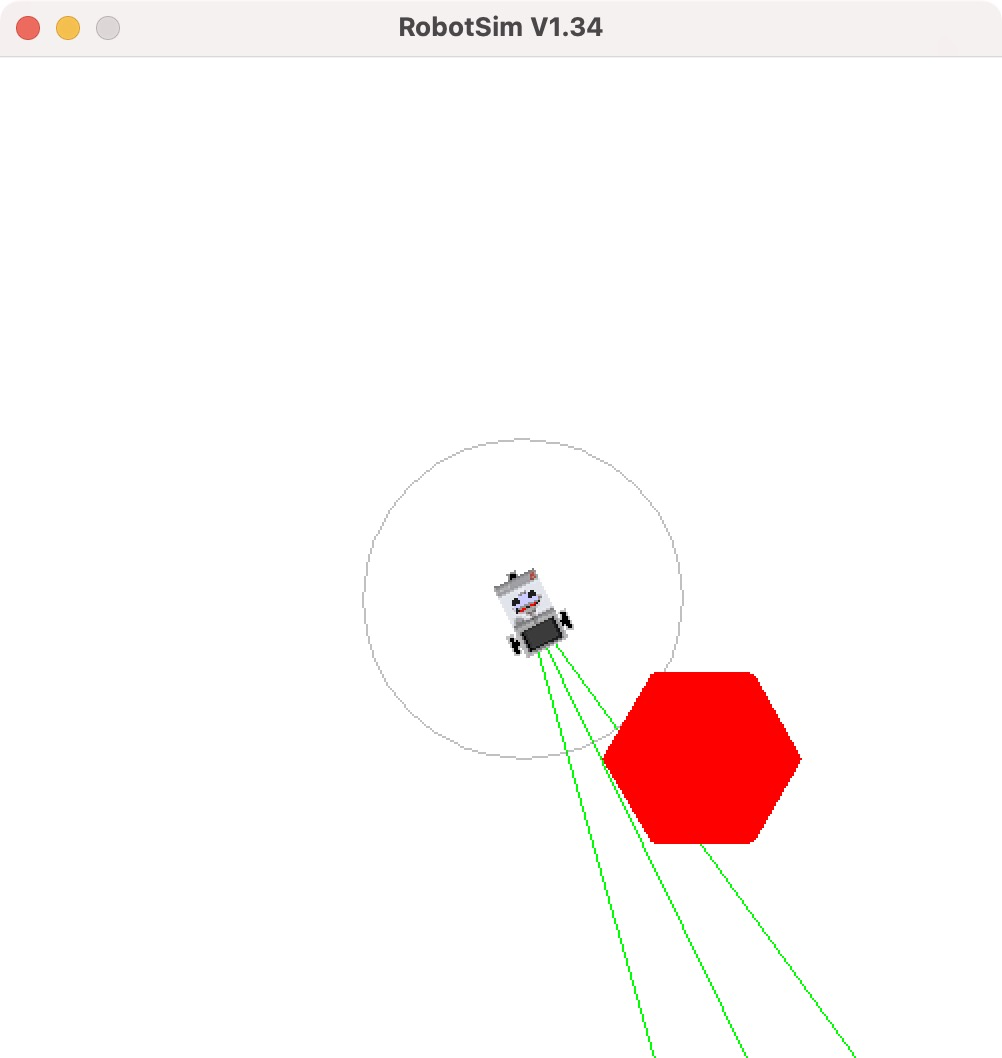
\includegraphics[width=0.5\textwidth]{images/result.jpg}
  \caption{Simulation Result}
  \label{fig:result}
\end{figure}


\subsection{Conclusion}
%\addcontentsline{toc}{subsection}{\protect\numberline{Conclusion}}%

In the pursuit of enhancing autonomous navigation and detection strategies, the utilization of ultrasonic sensors in a simulated environment has provided valuable insights. The simulation's focus on a two-dimensional ultrasonic sensor, equipped with the ability to measure distances to the nearest reflective targets within a defined cone, mirrors real-world scenarios where these sensors are pivotal.

By emulating the behavior of ultrasonic sensors, we've gained an appreciation for their radar-like capabilities, where beams of detection extend outward from the sensor's location. The concept of targets, represented by polygonal shapes and detected through a mesh of triangles, introduces a dynamic element to the detection process. The underlying distance detection algorithm has illuminated the intricacies of mapping distance to triangle intersections within the sensor's beam area.

Furthermore, the implementation of fixed target layouts using the \texttt{RobotContext} class showcases the adaptability of this technology to different operational modes. The continuity between simulated robot movement and real-world counterparts, be it direct interaction or autonomous navigation, underlines the practical significance of this simulation.

As we conclude this exploration, the simulation not only underscores the potential of ultrasonic sensors in spatial awareness and navigation but also paves the way for future studies. Beyond the confines of simulation, real-world applications beckon, offering solutions for diverse challenges ranging from robotic navigation to object detection and avoidance. The ability to dynamically modify targets and adapt to changing scenarios further emphasizes the flexibility and relevance of this technology.

This simulation has provided a glimpse into the world of ultrasonic sensors and their role in autonomous navigation. By unraveling the mechanics of distance detection, the simulation has set the stage for deeper investigations and real-world implementations that harness the power of ultrasonic sensors for more accurate and intelligent navigation systems.
